\chapter{Background \label{cpt: background}}

Our analysis is based on concepts from the \gls{ca}, a sub-field of linguistics, and is automated using tools and techniques from the \gls{nlp} area of computer science. This chapter first introduces all the \gls{nlp} concepts and tools used within this work (Sec. \ref{sec: nlp} to \ref{ssec: word embeddings}) and then all the linguistic concepts that our analysis is built on (Sec. \ref{sec: ca})
%and finally introduces work directly related to our project (Sec. ???).

\section{An Overview of Natural Language Processing \label{sec: nlp}}

Natural Language Processing (NLP) is a sub-field of computer science, artificial intelligence and linguistics, which attempts to use computers to analyse natural (human) language data. An example of advanced NLP applications are \textit{virtual assistants} such as the \textit{Google Home} or \textit{Amazon Alexa} devices, which need to understand queries spoken by a human (speech recognition), understand them (natural language understanding), execute the functionality that was asked for and formulate a response (natural language generation). The methods we apply fall firmly within the area of natural language understanding, as we apply (and modify) commonly used methods to the largely unexplored landscape of human conversations.

%NLP has had an increasingly important role and is commonly referenced as a key component to an \textit{artificial general intelligence} (AGI). CITE TURING.

Most NLP applications deal with low-noise text data, such as news articles, product reviews, or direct queries. Conversations between humans do not fall within this category and are associated with large amounts of noise: from members of the conversation talking over one-another to the use of sarcasm, jokes or slang, conversations are messy. For this reason, conversation analysis has largely been manual in nature. 
\section{Machine Learning \label{sec: ML}}
    A traditional computer programme takes some inputs $X$, does something with those inputs and outputs some output $Y$. It can be thought of as a function $f: X \rightarrow Y$. The behaviour of that function $f$ is defined by the programmer.
    %, who specifies what the computer is supposed to do with $X$ to turn it into $Y$.

    %The objective of \gls{ml} is to \textit{learn} the behaviour of such a function $f$ statistically as $\hat{f}$.
    In \gls{ml}, the behaviour of $\hat{f}$ is not implemented by a programmer, but statistically learned from data. $\hat{f}$ is called the \textbf{\gls{model}}. In practice, $\hat{f} = \hat{f}_\theta$ is highly flexible and its behaviour specified by a set of parameters $\theta$. These parameters are initially randomly assigned and then automatically tweaked until $\hat{f}_\theta$ shows the desired behaviour in a process called training (see Sec. \ref{ssec: training}).

    \gls{ml} is useful in cases that have too many inputs to be implemented traditionally, such as image recognition or \gls{nlp}.

    \subsection{Supervised Learning}
        In supervised learning, the \gls{ml} algorithm is fed pairs $(X, Y)$ of inputs $X$ and matching outputs $Y$ that were labelled manually by humans. If, for example, one wanted to train a \gls{model} that recognises cats, $X$ would be an image of a cat or an image not of a cat, and $Y$ would be the corresponding label \textit{cat} or \textit{not cat}. The algorithm uses $(X, Y)$ to iteratively compare its own prediction $\hat{f}_\theta(X) = \hat{Y}$ to the true output $Y$ and slightly adjusts its parameters $\theta$ to match that true output. This process is called training and the pairs of $(X, Y)$ accordingly are called training data. %There are many different approaches and implementations of the functions $\hat{f}_\theta$ and the training process. The type of $\hat{f}_\theta$ we use is called a \gls{nn} and it is trained through a process called backpropagation. We expand on this in section ???.
        Supervised learning is the main flavour of \gls{ml} used for this project.

    %\subsection{Unsupervised Learning}
        %In unsupervised learning, only the input data $X$ is provided (and no true labels $Y$). The \gls{ml} algorithm then uses some statistical techniques to provide some useful insights. The two main uses of unsupervised learning in this project are \gls{pca}, which reduces high-dimensional data to lower-dimensional data while trying to preserve similarity, and cluster analysis, which finds similarities within the datapoints $X$ and groups similar data-points together.
 
\section{Artificial Neural Networks \label{sec: neural nets}}

    \begin{figure}[h]
        \centering
        \begin{subfigure}[b]{0.9\textwidth}
            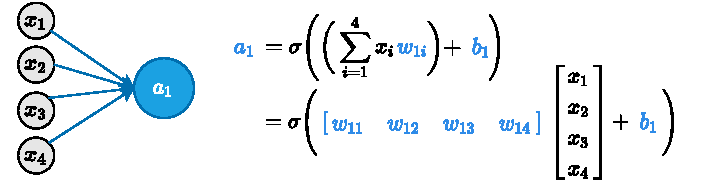
\includegraphics[width=\textwidth]{one_neuron.pdf}
            \caption{A single neuron connected to the input layer of 4 input neurons. It computes the activation function of the weighted sum of the previous layer's outputs as its own output. \label{subfig: neuron}}
        \end{subfigure}
        \hfill
        \begin{subfigure}[b]{0.9\textwidth}
            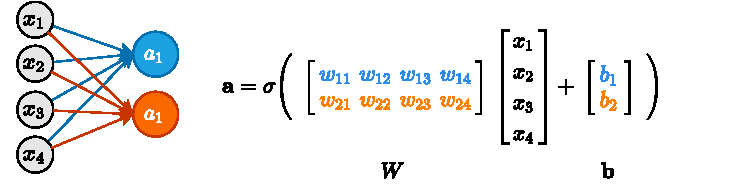
\includegraphics[width=\textwidth]{two_neurons.pdf}
            \caption{Using notation from linear algebra, the calculations computed by the whole layer (of two neurons) can be written as an activation function of a matrix multiplication and vector addition. \label{subfig: layer}}
        \end{subfigure}
        \caption{4 input neurons $x_i$ are connected to the next layer consisting of one neuron (a) or two neurons (b).}
    \end{figure}

    

    The models used for supervised learning throughout this project are called (artificial) neural networks (NNs). They are flexible information processing architectures (loosely) inspired by the network of neurons in the brain. It is not strictly necessary to understand the functionality of NNs to understand the rest of the project, simply noting that NNs are flexible functions $\hat{f}_{\theta} : X \rightarrow Y$ that can be trained to process information in the desired way using labelled training data $(X, Y)$ is enough. A quick introduction is however included for completeness.
    
    \subsection{Neurons}
        NNs are a connection of connected nodes called neurons that are sequentially organised into a number of layers. Each neuron contains a set of weights $w_i$ and a set of biases $b_i$ with $i \in [0, N_{in}]$, where $N_{in}$ is the number of inputs to that neuron. A neuron takes inputs $a_i^{(j)}$ from the previous layer $j$ and calculates its output as a weighted sum normalised by a non-linear \textit{activation function} $\sigma$ (see Sec. \ref{ssec: activation function}):
    
        \begin{equation}
            \label{eq: feed forward}
            a^{(j + 1)} = \sigma\bigg(\big(\sum_{i = 0}^{N_{in}} w_i a_i^{(j)}\big) + b\bigg).
        \end{equation}
        
        This output is the input for all connected neurons in the next layer, hence it is equal to $a^{(j+1)}$. This process of processing information is called the forward pass of the NN. A simple example of a neuron is shown in Fig. \ref{subfig: neuron}.
    
    \subsection{Layers}
        NNs are composed of multiple layers of multiple neurons. In many NNs, every neuron in layer $j$ is connected to every neuron in the next layer $j + 1$. We assume that this is the general case within this section. This allows for the use of linear algebra notation to simplify what each layer does.
        
        Writing the input vector of layer $j$ as $\mathbf{a}^{(j)}$, the weight matrix, containing all the weights of a neuron (column) for all neurons in a layer (row) as $W$ and the vector of biases of all neurons in a layer as $\mathbf{b}$ allows us to write the forward pass through each layer as
        
        \begin{equation}
            \mathbf{a}^{(j + 1)} = \sigma(W\mathbf{a}^{(j)} + \mathbf{b}),
        \end{equation}
        
        as \[
            \sigma\bigg( \big(x_0, x_1, \dots x_n) \bigg) = \bigg( \sigma(x_0), \sigma(x_1) \dots \sigma(x_n)\bigg). %todo make col vec
        \]
        
        A simple example, with only two layers can be found in Fig. \ref{subfig: layer}. The inputs to the first layer are the inputs to $\hat{f}_\theta$, $X$. The output(s) of the last layer are the predicted results $\hat{Y}$. 
        
        The information processing of a neural net with $N$ layers can thus be written as the repeated nested application of a weighted sum normalised at every layer $j$ by some $\sigma^{(j)}$:
        
        \begin{align}
            \label{eq: nested NN}
            \hat{\mathbf{Y}} = \mathbf{a}^{(N - 1)} &= \sigma^{(N-1)}\bigg(W^{(N - 1)}\mathbf{a}^{(N - 2)} + \mathbf{b}^{(N-1)}\bigg) \\
            &= \sigma^{(N-1)}\bigg(
                W^{(N - 1)}\big( \dots (
                \sigma^{(0)} \big(
                    W^{(0)} (\mathbf{X})) + \mathbf{b}^{(0)}
                    \big) \dots
                \big) + \mathbf{b}^{(N-1)} \nonumber
            \bigg).
        \end{align}
        
        The weights $W$ and biases $\mathbf{b}$ determine how the inputs $\mathbf{X}$ are processed to the outputs $\mathbf{Y}$ and are the parameters $\theta$ of the model. By inspecting Eq. \ref{eq: nested NN} and noting that every $W$ is a potentially large matrix and every $\mathbf{b}$ a potentially large vector of parameters, it is clear that the number of parameters grows quickly with the complexity of the NN's architecture (i.e. its number of neurons, and number of input features $\mathbf{X}$). It is not uncommon that the number of parameters exceeds 10s of millions for complex models. The state of the art language model, known as GPT-3 uses 175 billion parameters \cite{gpt3}. The training process, in which all of these parameters are tuned is explained in Sec. \ref{ssec: training}.
        
        The scale of complex NNs is also the reason why it is beneficial to frame computations as linear algebra operations: A computer's GPU (graphical processing unit) is capable of processing large numbers of repeated calculations much faster than central processing units (CPUs), by computing all required values in parallel\cite{herlihy2012art}. 
        Linear algebra computations (such as matrix multiplications and vector additions) are examples where highly parallel computation can accelerate computations significantly, reducing the time needed to process data using NNs significantly.\cite{herlihy2012art}
        
        \subsection{Activation Functions \label{ssec: activation function}}
    
        There are a number of different choices for the activation function $\sigma$. Most activation functions normalise values to lie within some fixed interval $(a_{min}, a_{max})$, i.e.
        \begin{equation}
        \sigma : x \rightarrow y, \hspace{3em} x \in [-\infty, \infty], y \in (a_{min}, a_{max}).
        \end{equation}
        
        Examples for $\sigma$ include $\tanh{x}$, $1/(1 + e^{-x})$, or the Heaviside step-function, each of which is used for different purposes.
        
        The normalisation provided by the activation function means that a small number of neurons can not dominate the final outcomes too heavily (known as the ``exploding gradients problem"). The second effect of these functions is the non-linearity they introduce, allowing for non-linear models for non-linear problems.
        
    \subsection{Training \label{ssec: training}}
        To train the NN is to determine a set of parameters $\theta$ that make the model map $X \rightarrow \hat{Y}$ in such a way that matches the provided \textit{true labels} $Y$. This is approached as an optimization problem, where the quantity minimised is called the loss.
        
        \subsubsection{Loss Function}
            The loss function maps predicted labels and true labels to the so-called loss $L$: \[\mathcal{L} : \hat{Y}, Y \rightarrow L.\] It is a measure of goodness of fit between the model's predictions and the true labels. One commonly used example is the mean-squared-error as the loss function:
            \[
                \mathcal{L} = \frac{\sum_{i = 1}^{n}(y_i - \hat{y}_i)^2}{n}, \hspace{2em} y_1 \dots y_n \in Y.
            \]
            
            Since $\hat{Y}$ depends on $\theta$, $\mathcal{L} = \mathcal{L}(\theta)$. Since $\mathcal{L}$ and $\sigma$ are both differentiable functions, partial derivatives of $\mathcal{L}$ with respect to $\theta$ can be calculated. 
        
        \subsubsection{Gradient Descent}
            By computing the gradient of $\nabla_\theta \mathcal{L}$ with respect to $\theta$, and slowly moving all weights towards the minimum along this gradient, a set of weights that minimises the $\mathcal{L}$ (and thus optimises the prediction) can be found. Writing all parameters $\theta$ as a vector $\boldsymbol{\theta}$, this gradient descent process can be written succinctly as
            
            \begin{equation}
                \boldsymbol{\theta} \rightarrow \boldsymbol{\theta} - \alpha \nabla_\theta \mathcal{L}(\boldsymbol{\theta}),
            \end{equation}
            
            repeated until convergence, where $\alpha << 1$ is the learning rate, chosen manually. 
\section{Neural Networks for Text Analysis \label{sec: NNs for text}}
    There are two key issues with using NNs for text-analysis:
    
    \begin{enumerate}
    \item NNs require equal-length inputs, but words and sentences can have variable lengths.
    \item NNs require $x_i \in X$ to be numbers, not words, sentences or characters. A simple map such as $a \rightarrow 1, b \rightarrow 2 \dots$ is worthless also, because words are arbitrary choices and don't have inherent meaning.
    \end{enumerate}
    

    The first issue is addressed by recurrent neural networks, see Sec. \ref{ssec: RNNs}.
    The second issue is addressed by so-called word-embeddings (Sec. \ref{ssec: word embeddings}) which lie at the heart of our project and NLP in general. 
\section{Recurrent Neural Networks \label{ssec: RNNs}}

    \begin{figure}[t]
        \centering
        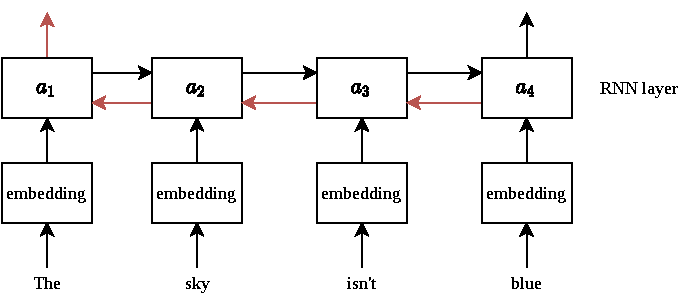
\includegraphics{rnn.pdf}
        \caption{The \gls{rnn} layer is given an input sequence of word \glspl{embedding}, calculates a hidden state depending on the first \gls{embedding} and the weights of the first neuron, and passes this hidden state on to the next \gls{neuron} within the \gls{rnn} layer. Every \gls{neuron} modifies the hidden state based on its weights and the input \gls{embedding} at its position and passes the modified state on. At the end of the sentence, the hidden state is passed on as the output of the layer. In a bidirectional \gls{model} (red arrows), a second hidden state is passed through the layer ``backwards".}
        \label{fig:rnn}
    \end{figure}
    Consider the following sentences as inputs to a \gls{nn}:

    \begin{table}[H]
    \begin{tabular}{|l|l|l|l|l|l|}
        \hline
        $i$   & 0   & 1   & 2     & 3    & 4    \\ \hline
        $s_1$ & The & sky & isn't & blue &      \\ \hline
        $s_2$ & The & sky & is    & blue &      \\ \hline
        $s_3$ & The & sky & is    & not  & blue \\ \hline
    \end{tabular}
    \centering
    \end{table}
    \noindent Using word \glspl{embedding} (see Sec. \ref{ssec: word embeddings}) we are able to turn these words into numbers that the \gls{nn} can process, but due to the (lack of) structure within sentences, we face another issue:
    Sentences $s_1$ and $s_2$ have different meanings, but because most words are the same, the inputs would appear relatively similar a hypothetical \gls{model} and yield similar outputs $\hat{Y}$. $s_1$ and $s_3$ have the same meaning, but are of different length. Therefore, in our hypothetical \gls{nn}, the inputs in positions $i = \{2, 3, 4\}$ are different, leading to potentially quite different outputs $\hat{Y}$.

    The problem is that in language, the absolute position of words within sentences is not particularly important, relative positions and context-words are: One word,``not", can change the meaning of the entire sentence dramatically.

     \Glspl{rnn} address these concerns and can process sequences of variable length such as sentences. \Glspl{rnn} use \glspl{neuron} as computational units in the same way traditional \glspl{nn} do, but instead of simply connecting \glspl{neuron} from the previous layer to \glspl{neuron} of the next layer, they connect \glspl{neuron} within a single layer, so that they form a directed graph. Every \gls{neuron} $n_i$ then corresponds to one entry in the sequence (e.g. one word in a sentence) and calculations are performed in a temporal direction: a hidden state of numbers is created at $n_1$, and repeatedly passed on to the next \gls{neuron} $n_{i+1}$, changed in a way determined by the $i+1$th entry and the \gls{neuron}'s parameters $\theta$ and passed on again. At the last \gls{neuron}, every entry has impacted the hidden state in some sensible way (specified by $\theta$) and the information can be passed to the next layer for further processing. A short example is given in Fig. \ref{fig:rnn}.


    \subsection{\gls{rnn} Architectures \label{ssec: rnn architectures}}
    The exact calculations that combine the hidden state with new inputs and parameters are determined by the internal structure of the \glspl{neuron}. The most prominently used \gls{neuron} architectures (which are also used in this project) are \gls{lstm}\cite{hochreiter1997long} and \gls{gru}\cite{chung2014empirical} architectures, both of which are capable of attaining state of the art performance on \gls{nlp} tasks\cite{huang2015bidirectional}.
    %%%%%%%%%%%%%%%%%%%

    \subsection{Bi-directional RNNs \label{ssec: bidirectional RNN}}
    If a \gls{rnn} layer is bi-directional, in addition to the hidden state being passed through the layer in a forward direction, another hidden state is passed through the layer backwards. This improves performance in many \gls{nlp} tasks, because e.g.  the impact of a given word on the meaning of a sentence does not only depend on its preceding, but also on its succeeding words. This means the \gls{rnn} layer has two outputs, one for the forwards pass and one for the backwards pass. This is indicated in red in Fig. \ref{fig:rnn}.

    \subsection{Outputting Hidden States \label{ssec: outputting hidden states}}
    In some cases, it is useful for the \gls{rnn} to have one output for every element in the sequence, not just one output at the end of the sequence. The different elements of the sequence still impact eachother's output, but now the output is a sequence of length equal to the input sequence. In that case, the hidden states of every \gls{neuron} are simply output to the next layer\cite{mlTextbook}.

    \subsubsection{When to Output Hidden States?}
    %Consider for example the following two different \glspl{model}, each with a different goal, but both taking a sequence of words $\mathcal{S}$ as an input.

    %The first \gls{model},
    %\begin{equation}
    %    \hat{f}_{\text{pos}}: \mathcal{S} \rightarrow \mathcal{P},
    %\end{equation}
    %outputs a sequence of \gls{pos} tags $\mathcal{P}$, one for every word e.g.
    %    \begin{equation*}
    %    \text{[The, house, is, green] $\rightarrow$ [article, %noun, verb, adjective]}.
    %    \end{equation*}
    %We still want the words to affect eachother's tags (i.e. green could be an adjective or a noun, depending on the other words in the sentence), but we want one tag for every word in the sequence. We want to map $N$ words $ \rightarrow N$ tags. In this case we want to return the $N$ hidden states as outputs.

    %The second \gls{model},
    %\begin{equation}
    %    \hat{f}_{q\Bar{q}}: \mathcal{S} \rightarrow q,
    %\end{equation}
    %outputs whether or not the sequence of words was a question or not, $q$. E.g.
    %    \begin{align*}
    %    \text{[The, house, is, green]} &\rightarrow \text{not a %question}\\
    %    \text{[Is, the, house, green]} &\rightarrow \text{question}.
    %    \end{align*}
    %It maps $N$ words $\rightarrow 1$ tag. In this case we want to output only one value, encapsulating the entire sequence; only the last \gls{neuron}'s value is returned.
    When we are mapping a sequence of length $N$ to a single tag (many to one) we only return the hidden state of the final \gls{neuron} encapsulating the entire sequence. When we instead map a sequence of length $N$ to an output sequence of tags of length $N$ instead, we return all hidden states.
 
\section[Conditional Random Fields]{Hidden Markov Models and Conditional Random Fields}

\Glspl{crf}\cite{originalCRF} are a graph-based modelling technique also used in sequence tagging commonly used in conjunction with \glspl{rnn} to improve classification accuracy. They can be understood as extensions to hidden Markov models.

\subsection{Hidden Markov Models}

    Hidden Markov models (HMMs) are based on markov processes. Markov processes describe a sequence of possible events in which the probability of each event depends \textit{only} on the state attained in the \textit{previous event}\cite{gagniuc2017markov}.
    HMMs consist of two such Markov processes: one process $\mathcal{X}$ with states that can be observed, such as a sequence of words, and one hidden process $\mathcal{Y}$ that depend on $\mathcal{X}$. The goal is to learn about $\mathcal{Y}$ by observing $\mathcal{X}$. HMMs use Bayesian modelling and apply them to Markov processes to make predictions\cite{klinger2007classical}.
   
   %TODO: Fix notation of $X, Y$ 
    \begin{figure}[t]
        \centering
        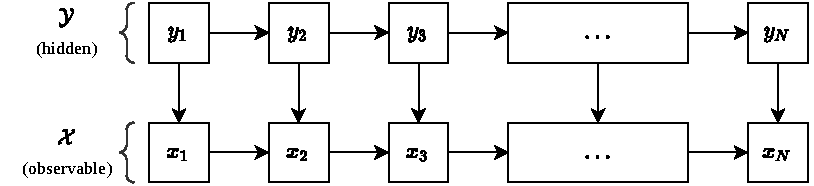
\includegraphics[width=0.90\textwidth]{hmm.pdf}
        \caption{In HMMs and CRFs, a hidden sequence $\mathcal{Y}$ is classified based on an an observable sequence $\mathcal{X}$.}
        \label{fig: HMM and CRF}
    \end{figure}

\subsection{Conditional Random Fields}
    \Glspl{crf} are a generalisation of HMM's that make fewer assumptions about probability distributions. Specifically, no assumptions on the dependencies among $x_{i} \in \mathcal{X}$ are made\cite{klinger2007classical}. Similar to how HMMs are Bayesian modelling applied to Markov processes, \glspl{crf} are an application of maximum entropy modelling to sequences\cite{klinger2007classical}.
\section{Word Embeddings \label{ssec: word embeddings}}

    \begin{figure}
        \centering
        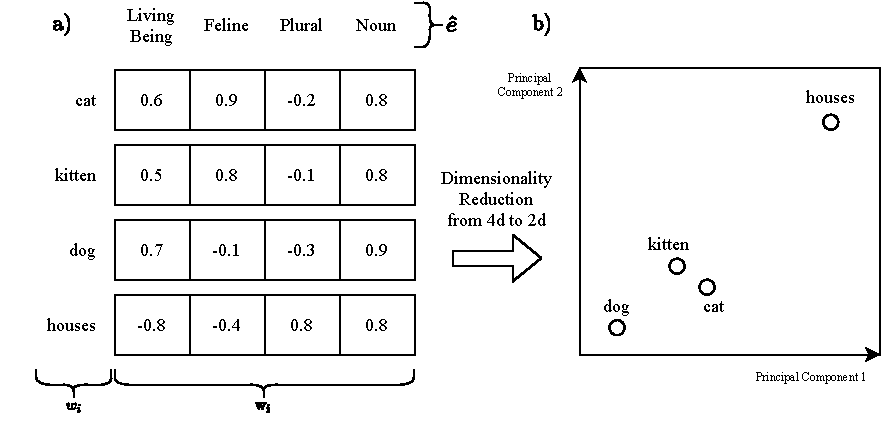
\includegraphics[width=0.9\textwidth]{embeddings.pdf}
        \caption{a) A schematic example of word \glspl{embedding} that represents each word in basis $\hat{e}$. In real-world embeddings, $\hat{e}$ is determined by the computer and has no human-understandable meaning. It also has much higher dimensionality. b) A graphical representation of the embedded words.}
        \label{fig:word embedding}
    \end{figure}

    For humans, (a large part of) learning a language is learning the mapping of words to their meanings such as ``dog" $\rightarrow$ pet with fur that makes ``woof" sound; ``table" $\rightarrow$ stable surface standing on legs etc. If a computer is to interpret textual information, we need to provide it with an analogous mapping. This is accomplished using word embeddings.
    Word \glspl{embedding} $\mathbf{w_i}$ are high-dimensional ($\approx 300$ dimensions) vectors of real numbers aiming to represent the semantic meaning of a word $w_i$. Fig. \ref{fig:word embedding} gives a simple example of such \glspl{embedding}. $\mathbf{w_i}$ are created by using large corpora of texts, (such as all Wikipedia articles, or a crawl through the entire internet) and using the context of words $w_i$ to learn their representation $\mathbf{w_i}$ in an unsupervised way. The basis for this is the assumption that similar words appear in similar contexts\cite{word2vec}.
    %Word \glspl{embedding} are at the heart of many \gls{nlp} applications and many pre-trained word \glspl{embedding} are available.
    The most prominent \glspl{embedding} are Google's, word2vec\cite{word2vec} and Stanford university's \gls{glove}\cite{glove} \glspl{embedding}. The lesser known \textit{ConceptNet Numberbatch} \glspl{embedding}\cite{conceptnet} build upon (and improve) both \gls{glove} and word2vec (see Sec. \ref{ssec: Numberbatch}).

    \subsection{GloVe \label{ssec: Glove}}
        \gls{glove}\cite{glove} (short for Global Vectors) is a mapping
        \[ \hat{f}(w_i) \rightarrow \mathbf{w_i}\]
        from words to \gls{embedding} vectors. It is trained on very large corpora such as Wikipedia or the entire internet. First, the co-occurence matrix $C_{ij}$ is created:

        \begin{equation}
        C_{ij} = \text{\# Co-occurences between words $i$ and $j$},
        \end{equation}

        where a co-occurence of two words means that they are featured within the same document, e.g. the same Wikipedia article or the same website. If there are $N_w$ words in the corpus, $C_{ij}$ is a $N_w \times N_w$ matrix, measuring the co-occurence between every word $w_i$ with every other word $w_j$.
        %For \gls{glove}, $N_w = \num{1.9e6}$ when trained on Wikipedia, $N_w = \num{2.2e6}$ when trained on a crawl of the entire internet.
        $C_{ij}$ is sparse, (meaning most entries are 0) as most words do not appear in the same context as most other words. By then performing dimensionality reduction (e.g. \gls{lda}) on $C_{ij}$, a dense representation of much lower dimensionality is obtained for every word. This representation is the word \gls{embedding}. For \gls{glove}, \glspl{embedding} are by default 300-dimensional\cite{glove}.

        Word2vec is trained in a similar way, though what counts as a co-occurence and how the dimensionality is reduced is slightly different\cite{word2vec}.

    \subsection{ConceptNet Numberbatch \label{ssec: Numberbatch}}

        ConceptNet is a open source semantic network that represents words (and short sequences of words commonly seen together) as nodes and the relationships between them as edges. An example is shown in Fig. \ref{fig: conceptnet}.
           \begin{figure}[h]
                \centering
                 \captionsetup{format=hang}
                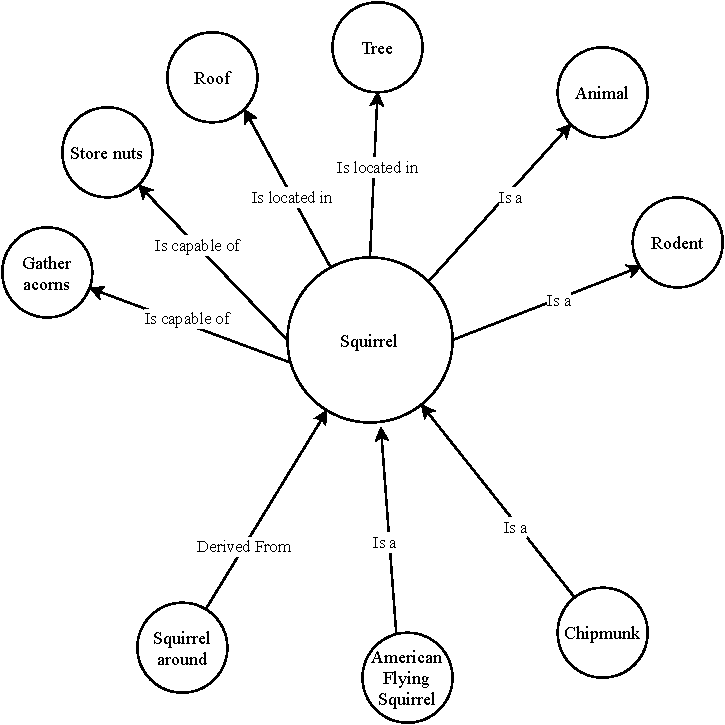
\includegraphics[width=0.7\textwidth]{conceptnet.pdf}
                \caption{Some of the connections of the word ``squirrel" in conceptNet. \label{fig: conceptnet}}
            \end{figure}

        By combining the ConceptNet network with other word \glspl{embedding} such as word2vec and \gls{glove} using a process called \textit{retrofitting}, a new, improved set of word \glspl{embedding}, the \textit{\gls{numberbatch}}, is created.

        \subsubsection{Retrofitting}
            Retrofitting uses a set of \glspl{embedding} $\mathbf{w_i}$, such as \gls{glove} or word2vec (Sec. \ref{ssec: Glove}) to infer new \glspl{embedding} $\Tilde{\mathbf{w_i}}$ that are both close to the original \glspl{embedding} and also close to their neighbours in the ConceptNet graph, by minimising the objective function
            \begin{equation}
                \Psi(W)=\sum_{i=1}^{N}\left[\alpha_{i}\left\|\mathbf{w}_{i}-\Tilde{\mathbf{w}}_{i}\right\|^{2}+\sum_{(i, j) \in E} \beta_{i j}\left\|\mathbf{w}_{i}-\mathbf{w}_{j}\right\|^{2}\right],
            \end{equation}
            where the sum is over all words included within the union of all words contained in ConceptNet with all words contained in the original \glspl{embedding}, $W$ is the set of all word \glspl{embedding} $\mathbf{w_i} \in W$, $E$ is the set of all edges within the ConceptNet graph, $\beta_{ij}$ is the weight of the edge between words $w_i$ and $w_j$ in the ConceptNet graph, and $\alpha_i$ are weights determining how important the previous \glspl{embedding} are compared to the edges within ConceptNet. How exactly $\alpha_i$ is determined is not explained within the original paper, but when a word is found within ConceptNet, that was not found within the \glspl{embedding}, $\alpha_i = 0$, allowing for a further expansion of the vocabulary.\cite{speer2017conceptnet}

        \subsubsection{Superior Performance}
            By combining word2vec, \gls{glove} and ConceptNet, the \gls{numberbatch} achieves superior performance in many word \gls{embedding} benchmarks\cite{speer2017conceptnet, conceptnetPerformance}.

        %\subsubsection{Mini Version}
            %As a convenience, the \gls{numberbatch} \glspl{embedding} are available as both more accurate 32-bit floating point numbers and as less accurate 8-bit integers. The 8-bit integer version allows for significantly smaller files (mini $\approx$ 50MB, full \glspl{embedding} $\approx$ 5GB) and loading times. We use the mini versions due to limited resources.

    \subsection{Similarity \label{ssec: cosine similarity}}
        The defining feature of word \glspl{embedding} is that semantically similar words have similar vectors. We can thus quantify the similarity $\eta_{ij}$ between two words $w_i, w_j$ as the cosine similarity of their \glspl{embedding}
        \begin{equation}
            \eta_{ij} = \text{cosine}(\mathbf{w_i}, \mathbf{w_j}) = \frac{\mathbf{w_i} \cdot \mathbf{w_j}}{|\mathbf{w_i}| |\mathbf{w_j}|}.
            \label{eq: cosine similarity}
        \end{equation}
        We use this notion of similarity heavily in this work.

    \subsection{Sentence Embeddings \label{ssec: utterance embeddings}}

    In the same way that words can be embedded based on a pre-trained set of \glspl{embedding}, sentences can be embedded also. Training the \glspl{embedding} doesn't work in the same way as for words (otherwise every sentence would have to be contained within the corpus for an \gls{embedding} to exist), but the concept is the same. A sentence is represented as a vector in a high-dimensional vector space. This allows a similarity between sentences to be computed as the cosine similarity (see Sec. \ref{ssec: cosine similarity}, Eq. \ref{eq: cosine similarity}). Examples include Google's universal sentence encoder\cite{GoogleEncoder} and Facebook's InferSent\cite{infersent}.

    \subsection{Limitations}
        \begin{figure}[h]
            \centering
            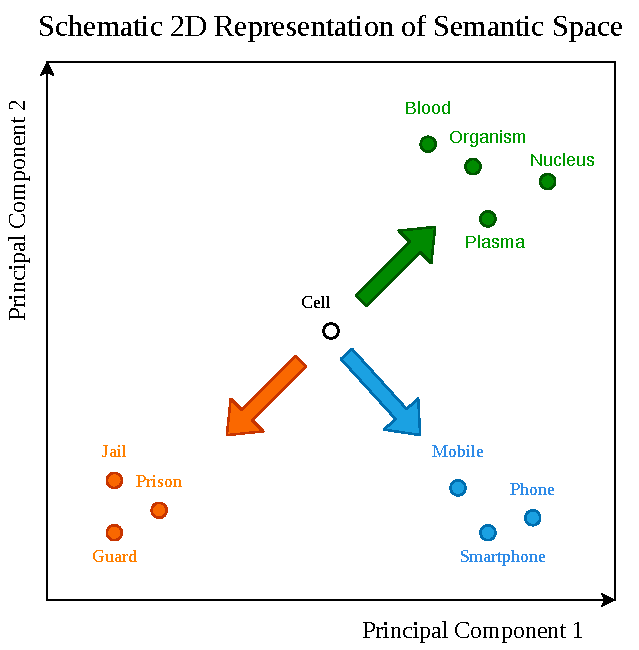
\includegraphics{ambiguous_embedding.pdf}
            \caption{Due to appearing frequently in contexts relating to biology, phones and prison, the word \gls{embedding} for the ambiguous word ``cell" is attracted to all three contexts in semantic space. The final \gls{embedding} lies somewhere in between the contexts and is a poor representation for all three meanings of ``cell".}
            \label{fig:ambiguous_embedding}
        \end{figure}

        Word \glspl{embedding} suffer from some limitations, the most significant of which is the problem of word-sense disambiguation, which occurs because words may have multiple meanings but only one \gls{embedding}. In the sentence
        \begin{align*}
            &\textit{``He went to the prison cell with his cell phone to extract blood cell samples}\\
            & \textit{from the inmates."}
        \end{align*}
        the word \textit{cell} appears 3 times and has a different meaning every time, but it has only one word \gls{embedding}. Because the method of \gls{embedding} is incapable of disambiguating the different meanings of the words, the word \gls{embedding} is poor: In the semantic vector space of word \glspl{embedding}, \textit{cell} will be attracted to words within its ``biology context", but also within its ``phone" context and within its ``prison" context, leading to a final \gls{embedding} somewhere in the middle, making it ineffective within all three contexts. The newest types of word \glspl{embedding}, such as BERT\cite{devlin2018bert} or ELMo\cite{peters2018elmo} address this problem by taking whole sentences as inputs and use the context of adjacent words to compute disambiguated word \glspl{embedding}.

\section{Conversation Analysis \label{sec: ca}}
\glsreset{ca}
The analysis of the structure of conversations falls within the field of \gls{ca}, a sub-field of linguistics. This section explores the key concepts from \gls{ca} that we use for our work. 
% CONVERSATION ANALYSIS FIRST
    \subsection{Utterances \label{ssec: utterances}}
        Within conversations, \glspl{utterance} are strings of words that begin and end with a clear pause. As an approximation, we are assuming that every \gls{utterance} corresponds to a sentence and in this thesis, sentences and \glspl{utterance} are considered synonyms.
        
        
    \subsection{Dialogue Acts \label{ssec: DAs}}
        The atomic unit within \gls{ca} is the \gls{da}. The \gls{da} describes the \textit{social action} of an \gls{utterance}. \Glspl{da} can be split into categories such as questions, greetings, statements of politeness, statements of agreement etc. for our work, we use the SWBD-DAMSL tag-set of 42 \glspl{da} featured in the \gls{swda} corpus (see Sec. \ref{ssec: swda})\cite{fang2012annotation, swda}. The most common \glspl{da} as well as their relative frequency within the \gls{swda} corpus is shown in table \ref{table: damsl das}.
        
        \begin{table}[ht]
        \begin{tabular}{|l|l|l|}
        \hline
            \textbf{SWBD-DAMSL}          & \textbf{Example}                                & \textbf{\%} \\ \hline
            Statement-non-opinion        & Me, I'm in the legal department.                & 36\%        \\ \hline
            Acknowledge (Backchannel)    & Uh-huh.                                         & 19\%        \\ \hline
            Statement-opinion            & I think it's great                              & 13\%        \\ \hline
            Agree/Accept                 & That's exactly it.                              & 5\%         \\ \hline
            Abandoned or Turn-Exit       & So, -                                           & 5\%         \\ \hline
            Appreciation                 & I can imagine.                                  & 2\%         \\ \hline
            Yes-No-Question              & Do you have to have any special training?       & 2\%         \\ \hline
            Non-verbal                   & {[}Laughter{]}, {[}Throat\_clearing{]}          & 2\%         \\ \hline
            Yes answers                  & Yes.                                            & 1\%         \\ \hline
            Conventional-closing         & Well, it's been nice talking to you.            & 1\%         \\ \hline
            Uninterpretable              & But, uh, yeah                                   & 1\%         \\ \hline
            Wh-Question                  & Well, how old are you?                          & 1\%         \\ \hline
            No answers                   & No.                                             & 1\%         \\ \hline
            Response Acknowledgement     & Oh, okay.                                       & 1\%         \\ \hline
            Hedge                        & I don't know if I'm making any sense or not.    & 1\%         \\ \hline
            Declarative Yes-No-Question  & So you can afford to get a house?               & 1\%         \\ \hline
            Other                        & Well give me a break, you know.                 & 1\%         \\ \hline
            Backchannel in question form & Is that right?                                  & 1\%         \\ \hline
            Quotation                    & You can't be pregnant and have cats             & .5\%        \\ \hline
            Summarize/reformulate        & Oh, you mean you went home.                     & .5\%        \\ \hline
            Affirmative non-yes answers  & It is.                                          & .4\%        \\ \hline
        \end{tabular}
        \caption{The most common SWBD-DAMSL dialogue acts, taken from \cite{swda}. The third column is the fractional frequency of the DA within the \gls{swda} corpus of short conversations (see Sec. \ref{ssec: swda}).}
        \label{table: damsl das}
        \end{table} 
        

    
    %\subsection{Adjacency Pairs \label{ssec: adjacency pairs}}
        
        %In a conversation, speech acts are part of a greater cohesive structure. In \gls{ca}, this is the structure of \textit{adjacency pairs}. Adjacency pairs are pairs of speech acts $(s_j, s_{j+1})$, in which the initial speech act with label $s_j$ is replied to by the response with label $s_{j+1}$. Examples include:
        %\begin{itemize}
        %    \item (question, answer)
        %    \item (greeting, greeting)
        %    \item (request, denial)
        %    \item (opinion, agreement) etc.
        %\end{itemize}
        %A conversation, on the \gls{utterance} level, is structured as a long string of such adjacency pairs.
        
    
    
\glsresetall
